% Options for packages loaded elsewhere
\PassOptionsToPackage{unicode}{hyperref}
\PassOptionsToPackage{hyphens}{url}
\PassOptionsToPackage{dvipsnames,svgnames,x11names}{xcolor}
%
\documentclass[
  letterpaper,
  DIV=11,
  numbers=noendperiod]{scrartcl}

\usepackage{amsmath,amssymb}
\usepackage{lmodern}
\usepackage{iftex}
\ifPDFTeX
  \usepackage[T1]{fontenc}
  \usepackage[utf8]{inputenc}
  \usepackage{textcomp} % provide euro and other symbols
\else % if luatex or xetex
  \usepackage{unicode-math}
  \defaultfontfeatures{Scale=MatchLowercase}
  \defaultfontfeatures[\rmfamily]{Ligatures=TeX,Scale=1}
\fi
% Use upquote if available, for straight quotes in verbatim environments
\IfFileExists{upquote.sty}{\usepackage{upquote}}{}
\IfFileExists{microtype.sty}{% use microtype if available
  \usepackage[]{microtype}
  \UseMicrotypeSet[protrusion]{basicmath} % disable protrusion for tt fonts
}{}
\makeatletter
\@ifundefined{KOMAClassName}{% if non-KOMA class
  \IfFileExists{parskip.sty}{%
    \usepackage{parskip}
  }{% else
    \setlength{\parindent}{0pt}
    \setlength{\parskip}{6pt plus 2pt minus 1pt}}
}{% if KOMA class
  \KOMAoptions{parskip=half}}
\makeatother
\usepackage{xcolor}
\setlength{\emergencystretch}{3em} % prevent overfull lines
\setcounter{secnumdepth}{-\maxdimen} % remove section numbering
% Make \paragraph and \subparagraph free-standing
\ifx\paragraph\undefined\else
  \let\oldparagraph\paragraph
  \renewcommand{\paragraph}[1]{\oldparagraph{#1}\mbox{}}
\fi
\ifx\subparagraph\undefined\else
  \let\oldsubparagraph\subparagraph
  \renewcommand{\subparagraph}[1]{\oldsubparagraph{#1}\mbox{}}
\fi


\providecommand{\tightlist}{%
  \setlength{\itemsep}{0pt}\setlength{\parskip}{0pt}}\usepackage{longtable,booktabs,array}
\usepackage{calc} % for calculating minipage widths
% Correct order of tables after \paragraph or \subparagraph
\usepackage{etoolbox}
\makeatletter
\patchcmd\longtable{\par}{\if@noskipsec\mbox{}\fi\par}{}{}
\makeatother
% Allow footnotes in longtable head/foot
\IfFileExists{footnotehyper.sty}{\usepackage{footnotehyper}}{\usepackage{footnote}}
\makesavenoteenv{longtable}
\usepackage{graphicx}
\makeatletter
\def\maxwidth{\ifdim\Gin@nat@width>\linewidth\linewidth\else\Gin@nat@width\fi}
\def\maxheight{\ifdim\Gin@nat@height>\textheight\textheight\else\Gin@nat@height\fi}
\makeatother
% Scale images if necessary, so that they will not overflow the page
% margins by default, and it is still possible to overwrite the defaults
% using explicit options in \includegraphics[width, height, ...]{}
\setkeys{Gin}{width=\maxwidth,height=\maxheight,keepaspectratio}
% Set default figure placement to htbp
\makeatletter
\def\fps@figure{htbp}
\makeatother

\KOMAoption{captions}{tableheading}
\makeatletter
\@ifpackageloaded{tcolorbox}{}{\usepackage[many]{tcolorbox}}
\@ifpackageloaded{fontawesome5}{}{\usepackage{fontawesome5}}
\definecolor{quarto-callout-color}{HTML}{909090}
\definecolor{quarto-callout-note-color}{HTML}{0758E5}
\definecolor{quarto-callout-important-color}{HTML}{CC1914}
\definecolor{quarto-callout-warning-color}{HTML}{EB9113}
\definecolor{quarto-callout-tip-color}{HTML}{00A047}
\definecolor{quarto-callout-caution-color}{HTML}{FC5300}
\definecolor{quarto-callout-color-frame}{HTML}{acacac}
\definecolor{quarto-callout-note-color-frame}{HTML}{4582ec}
\definecolor{quarto-callout-important-color-frame}{HTML}{d9534f}
\definecolor{quarto-callout-warning-color-frame}{HTML}{f0ad4e}
\definecolor{quarto-callout-tip-color-frame}{HTML}{02b875}
\definecolor{quarto-callout-caution-color-frame}{HTML}{fd7e14}
\makeatother
\makeatletter
\makeatother
\makeatletter
\makeatother
\makeatletter
\@ifpackageloaded{caption}{}{\usepackage{caption}}
\AtBeginDocument{%
\ifdefined\contentsname
  \renewcommand*\contentsname{Table of contents}
\else
  \newcommand\contentsname{Table of contents}
\fi
\ifdefined\listfigurename
  \renewcommand*\listfigurename{List of Figures}
\else
  \newcommand\listfigurename{List of Figures}
\fi
\ifdefined\listtablename
  \renewcommand*\listtablename{List of Tables}
\else
  \newcommand\listtablename{List of Tables}
\fi
\ifdefined\figurename
  \renewcommand*\figurename{Figure}
\else
  \newcommand\figurename{Figure}
\fi
\ifdefined\tablename
  \renewcommand*\tablename{Table}
\else
  \newcommand\tablename{Table}
\fi
}
\@ifpackageloaded{float}{}{\usepackage{float}}
\floatstyle{ruled}
\@ifundefined{c@chapter}{\newfloat{codelisting}{h}{lop}}{\newfloat{codelisting}{h}{lop}[chapter]}
\floatname{codelisting}{Listing}
\newcommand*\listoflistings{\listof{codelisting}{List of Listings}}
\makeatother
\makeatletter
\@ifpackageloaded{caption}{}{\usepackage{caption}}
\@ifpackageloaded{subcaption}{}{\usepackage{subcaption}}
\makeatother
\makeatletter
\@ifpackageloaded{tcolorbox}{}{\usepackage[many]{tcolorbox}}
\makeatother
\makeatletter
\@ifundefined{shadecolor}{\definecolor{shadecolor}{rgb}{.97, .97, .97}}
\makeatother
\makeatletter
\makeatother
\ifLuaTeX
  \usepackage{selnolig}  % disable illegal ligatures
\fi
\IfFileExists{bookmark.sty}{\usepackage{bookmark}}{\usepackage{hyperref}}
\IfFileExists{xurl.sty}{\usepackage{xurl}}{} % add URL line breaks if available
\urlstyle{same} % disable monospaced font for URLs
\hypersetup{
  pdftitle={QGIS\_1},
  colorlinks=true,
  linkcolor={blue},
  filecolor={Maroon},
  citecolor={Blue},
  urlcolor={Blue},
  pdfcreator={LaTeX via pandoc}}

\title{QGIS\_1}
\author{}
\date{}

\begin{document}
\maketitle
\ifdefined\Shaded\renewenvironment{Shaded}{\begin{tcolorbox}[breakable, boxrule=0pt, interior hidden, enhanced, frame hidden, borderline west={3pt}{0pt}{shadecolor}, sharp corners]}{\end{tcolorbox}}\fi

\hypertarget{qgis-tasks}{%
\subsection{QGIS tasks}\label{qgis-tasks}}

\hypertarget{i-read-data}{%
\subsubsection{I) Read data}\label{i-read-data}}

\begin{itemize}
\item
  \textbf{Point data (.csv)} Open a Delimited Text Layer

  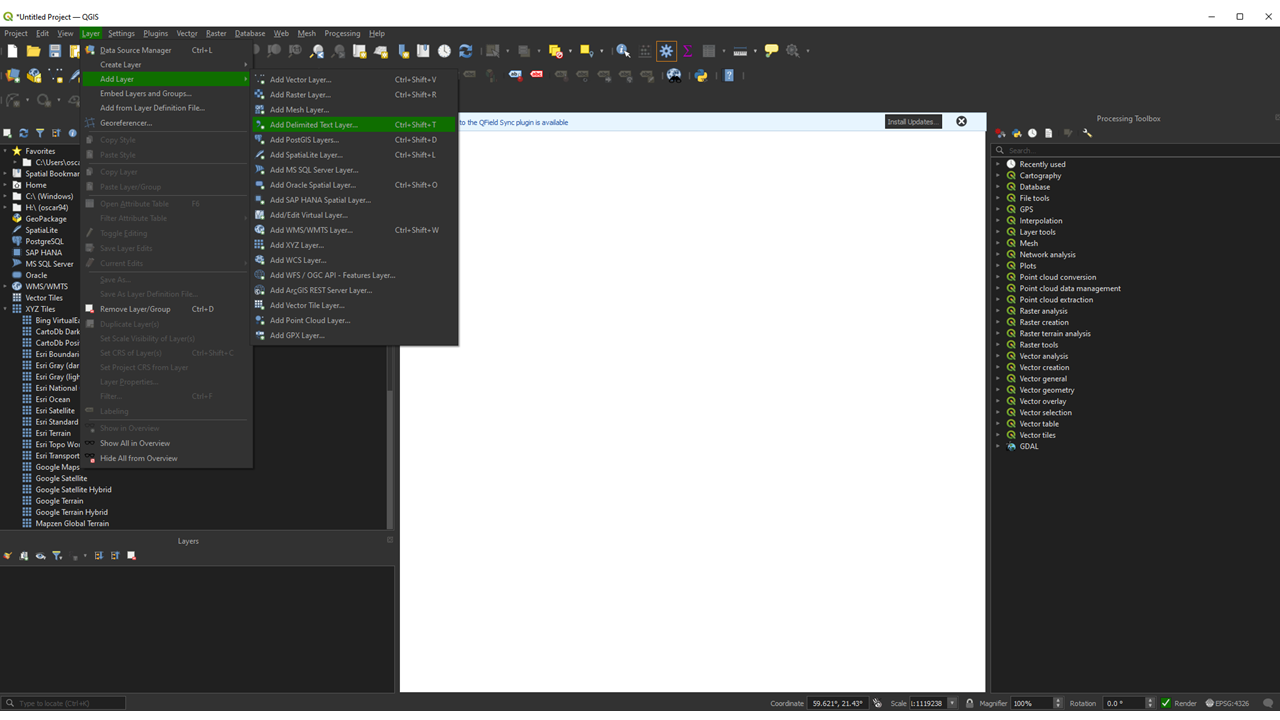
\includegraphics{Lab1/qgis_ss/QGIS_ss1.png}

  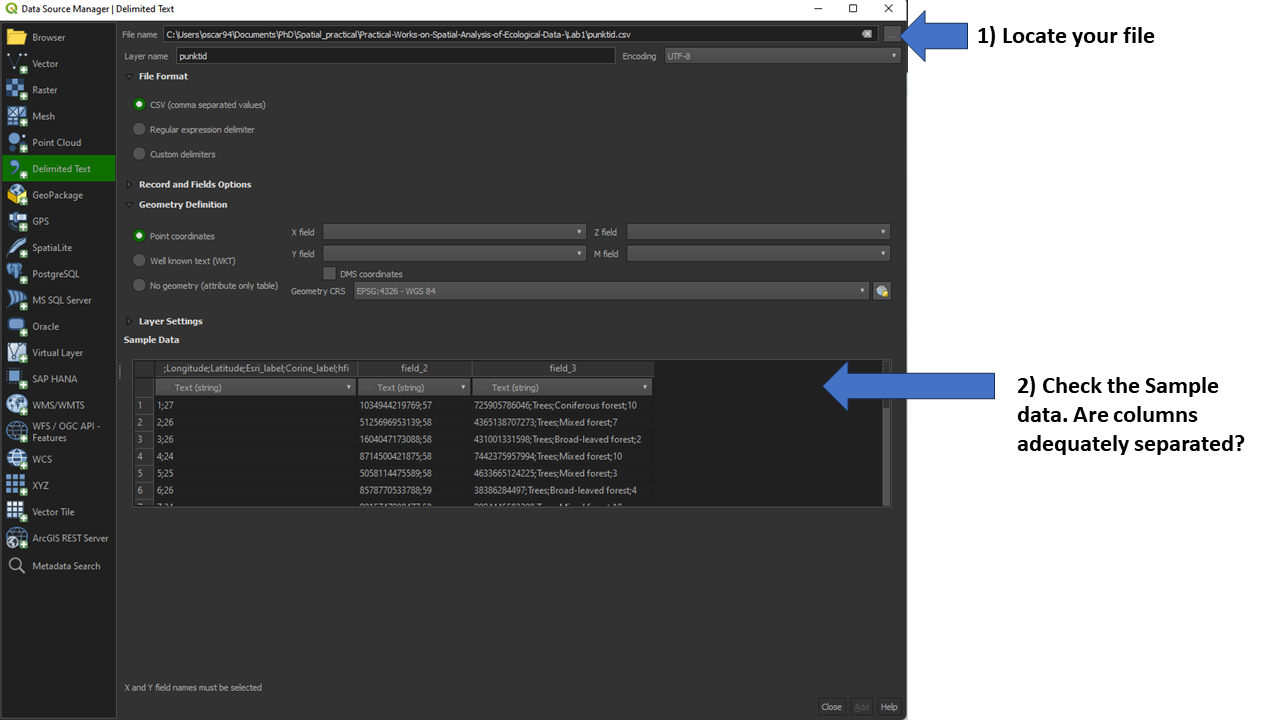
\includegraphics{Lab1/qgis_ss/QGIS_ss2.png}
\end{itemize}

\begin{tcolorbox}[enhanced jigsaw, colbacktitle=quarto-callout-tip-color!10!white, toptitle=1mm, opacityback=0, bottomtitle=1mm, bottomrule=.15mm, leftrule=.75mm, coltitle=black, left=2mm, arc=.35mm, title=\textcolor{quarto-callout-tip-color}{\faLightbulb}\hspace{0.5em}{Tip}, breakable, colframe=quarto-callout-tip-color-frame, opacitybacktitle=0.6, rightrule=.15mm, toprule=.15mm, titlerule=0mm, colback=white]
Check text delimiter (\textbf{,} , \textbf{;} , * *, \ldots) in notepad
\end{tcolorbox}

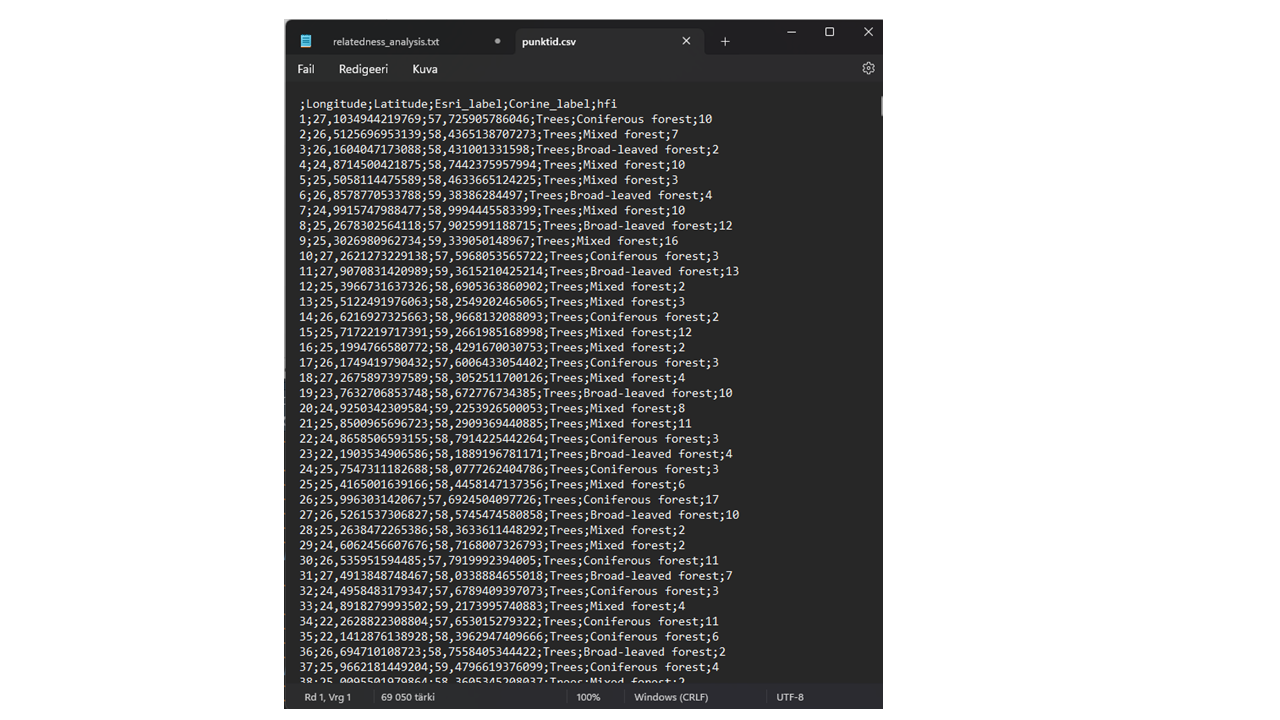
\includegraphics{Lab1/qgis_ss/QGIS_ss3.png}

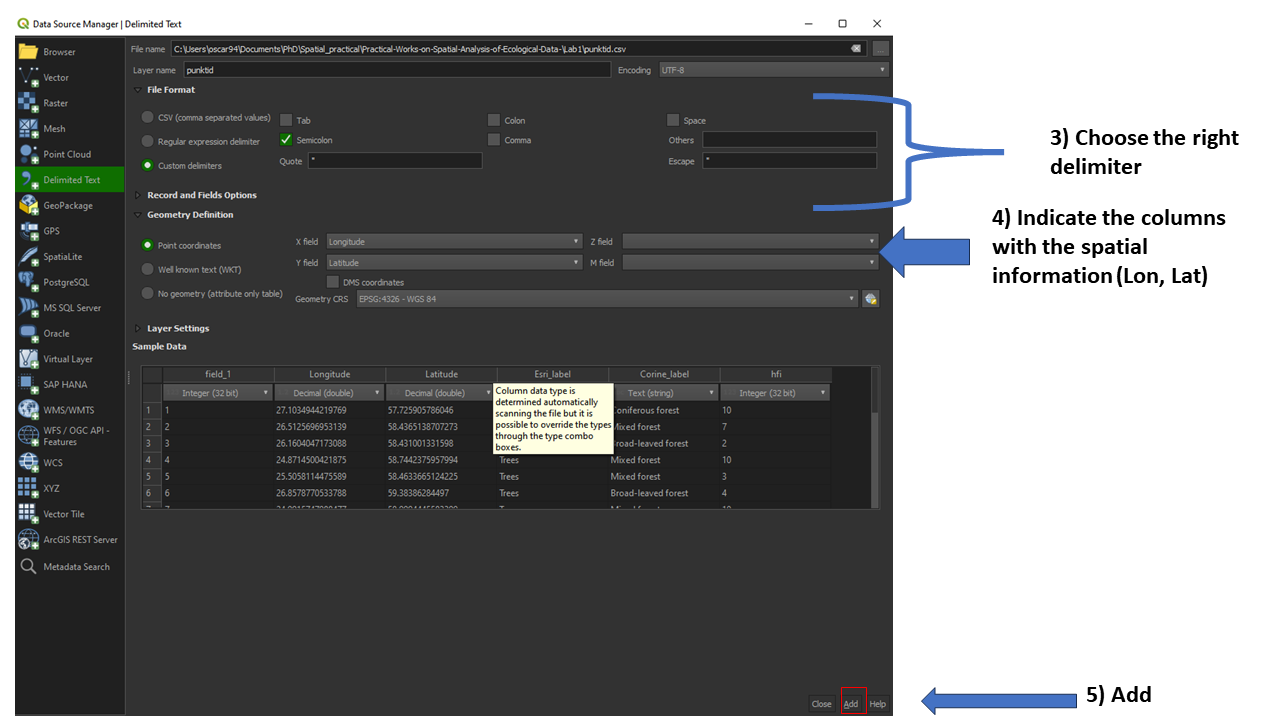
\includegraphics{Lab1/qgis_ss/QGIS_ss4.png}

\begin{tcolorbox}[enhanced jigsaw, colbacktitle=quarto-callout-warning-color!10!white, toptitle=1mm, opacityback=0, bottomtitle=1mm, bottomrule=.15mm, leftrule=.75mm, coltitle=black, left=2mm, arc=.35mm, title=\textcolor{quarto-callout-warning-color}{\faExclamationTriangle}\hspace{0.5em}{NB!}, breakable, colframe=quarto-callout-warning-color-frame, opacitybacktitle=0.6, rightrule=.15mm, toprule=.15mm, titlerule=0mm, colback=white]
Depending on your computer and language settings, the decimal separator
might be a comma (,) or point (.). The file uses comma as decimal
separator, if your computer uses point the file won't be read properly.
\end{tcolorbox}

If all was done correctly you should see it:
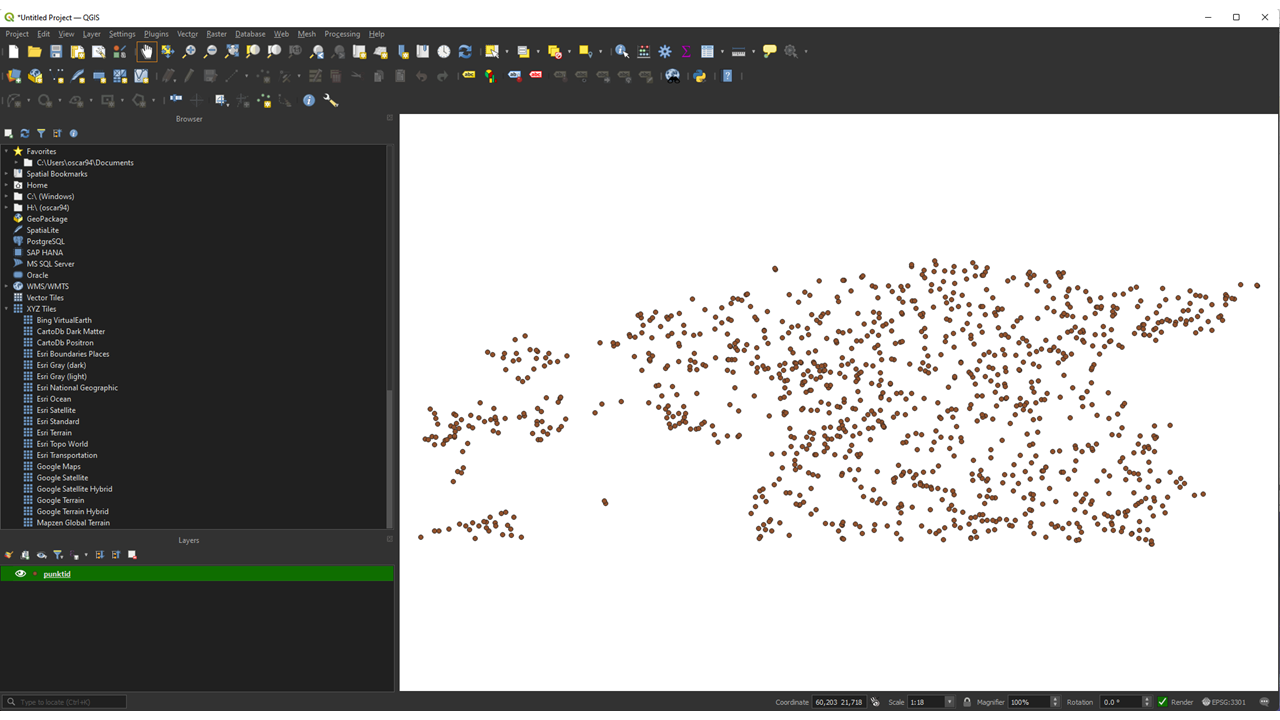
\includegraphics{Lab1/qgis_ss/QGIS_ss5.png}

\begin{itemize}
\tightlist
\item
  \textbf{Vector data}
\end{itemize}

Easiest way is just to drag the file (.shp) from the folder.

\includegraphics{Lab1/qgis_ss/gif_1.gif}

\begin{itemize}
\tightlist
\item
  \textbf{Raster data}
\end{itemize}

Drag them from the folder just like the vector data, or also from the
\textbf{layer} menu

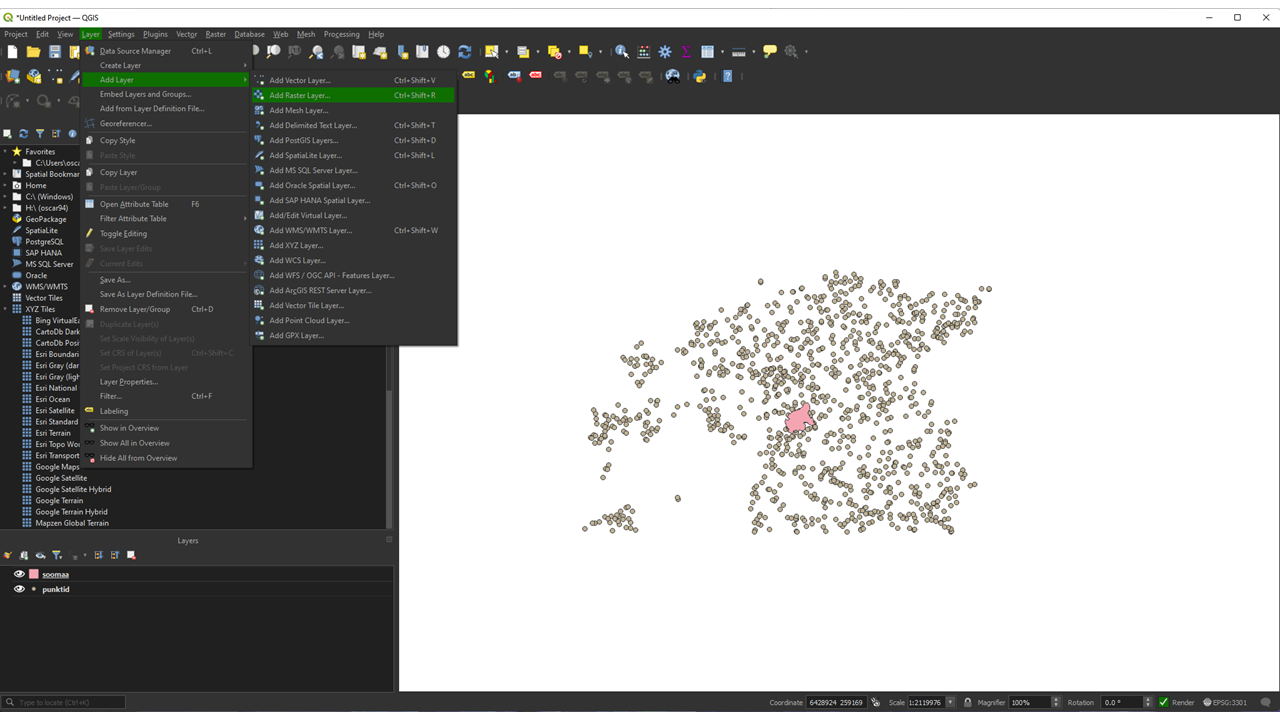
\includegraphics{Lab1/qgis_ss/QGIS_ss6.png}

You should see the 3 layers 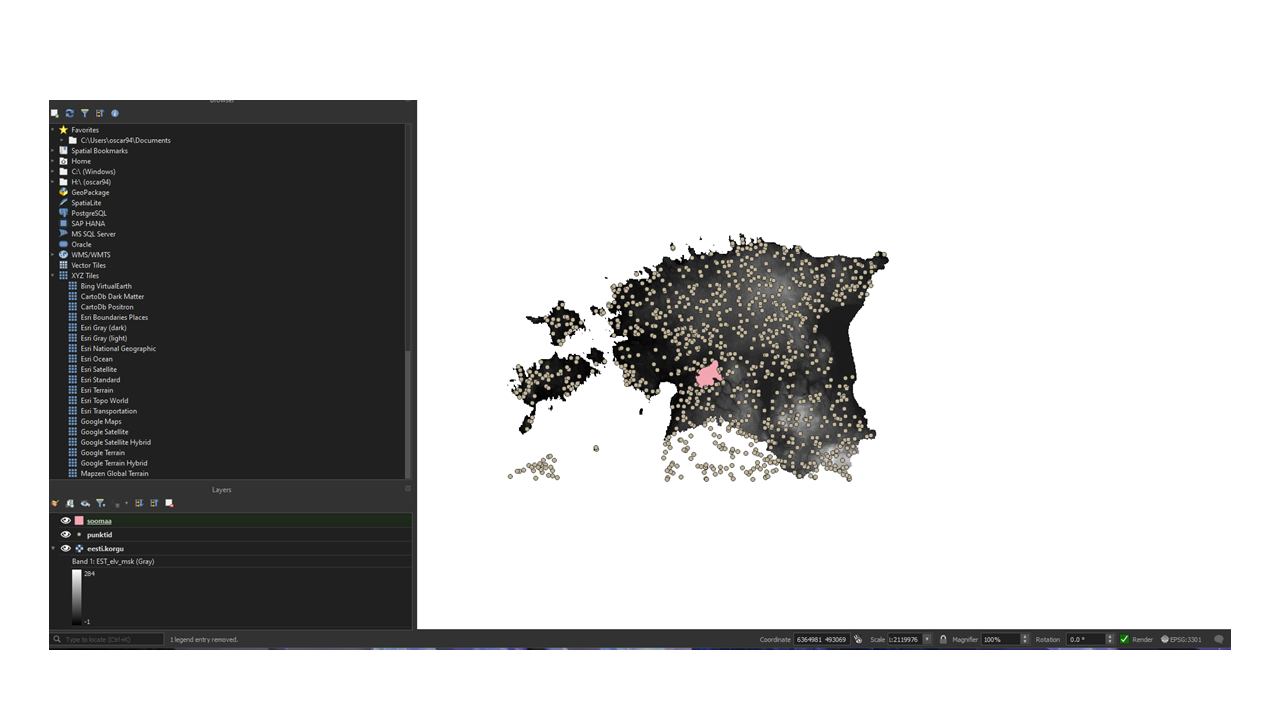
\includegraphics{Lab1/qgis_ss/QGIS_ss7.png}

\hypertarget{ii-check-properties-of-layers.}{%
\subsection{II) Check properties of
layers.}\label{ii-check-properties-of-layers.}}

\begin{itemize}
\tightlist
\item
  Right click and open properties of the layer
\end{itemize}

\includegraphics{Lab1/qgis_ss/gif_2.gif}

\begin{itemize}
\tightlist
\item
  Right click on the point layer to open the attributes table
\end{itemize}

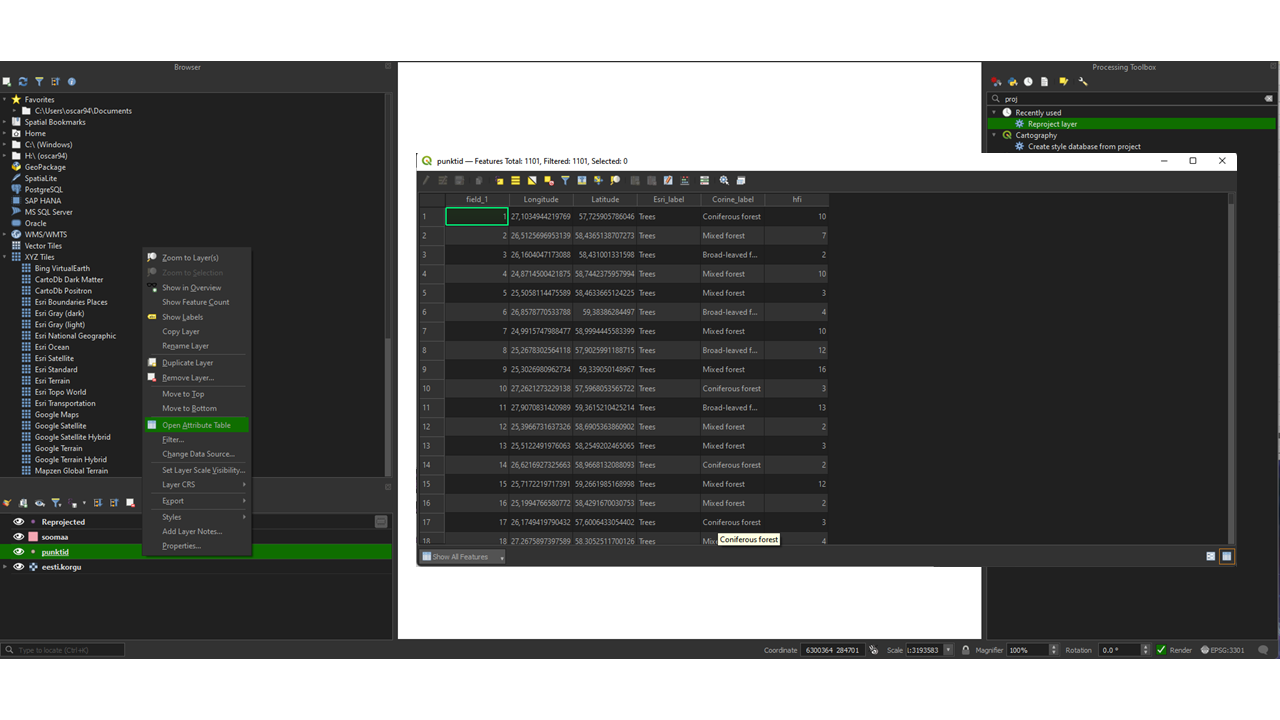
\includegraphics{Lab1/qgis_ss/QGIS_ss10.png}

\begin{itemize}
\tightlist
\item
  Change symbology base on columns
\end{itemize}

\begin{enumerate}
\def\labelenumi{\arabic{enumi})}
\tightlist
\item
  Right click on the layer
\item
  Open layer properties
\item
  Symbology
\item
  Choose proper settings and a column to symbolize it
\item
  Click \textbf{Classify} and \textbf{Apply}
\end{enumerate}

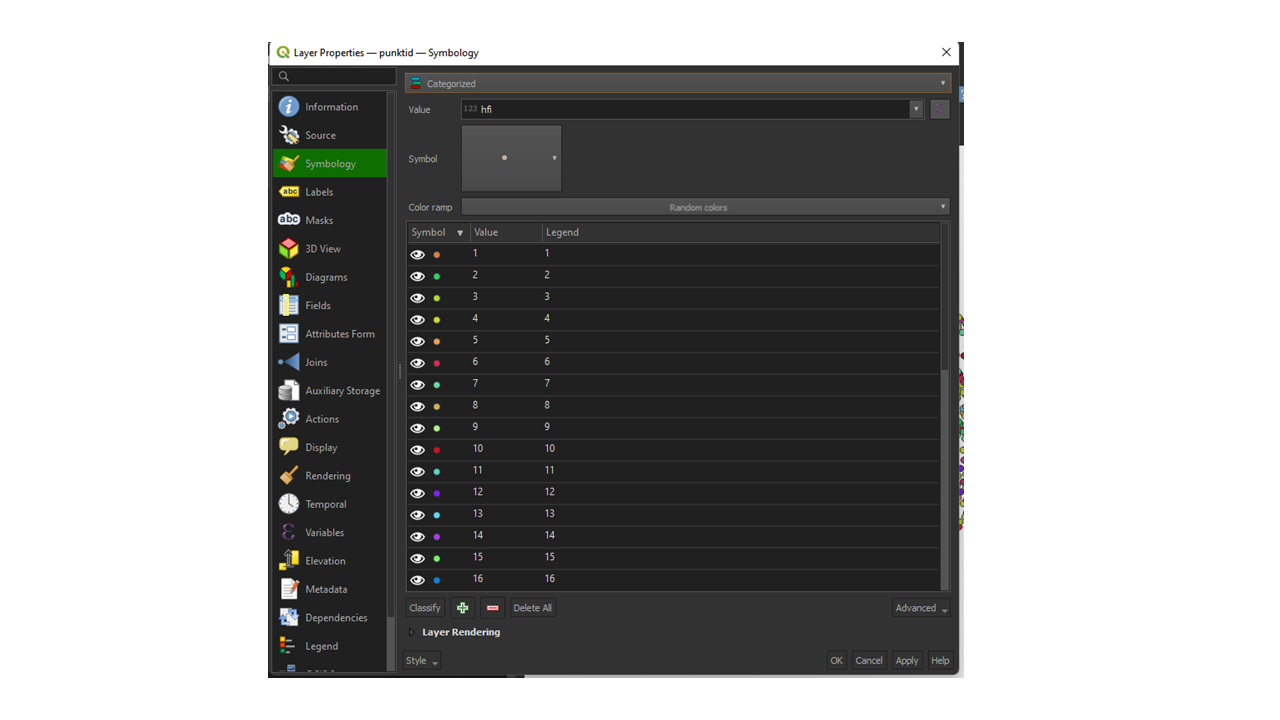
\includegraphics{Lab1/qgis_ss/QGIS_ss11.png} Look how symbology changes

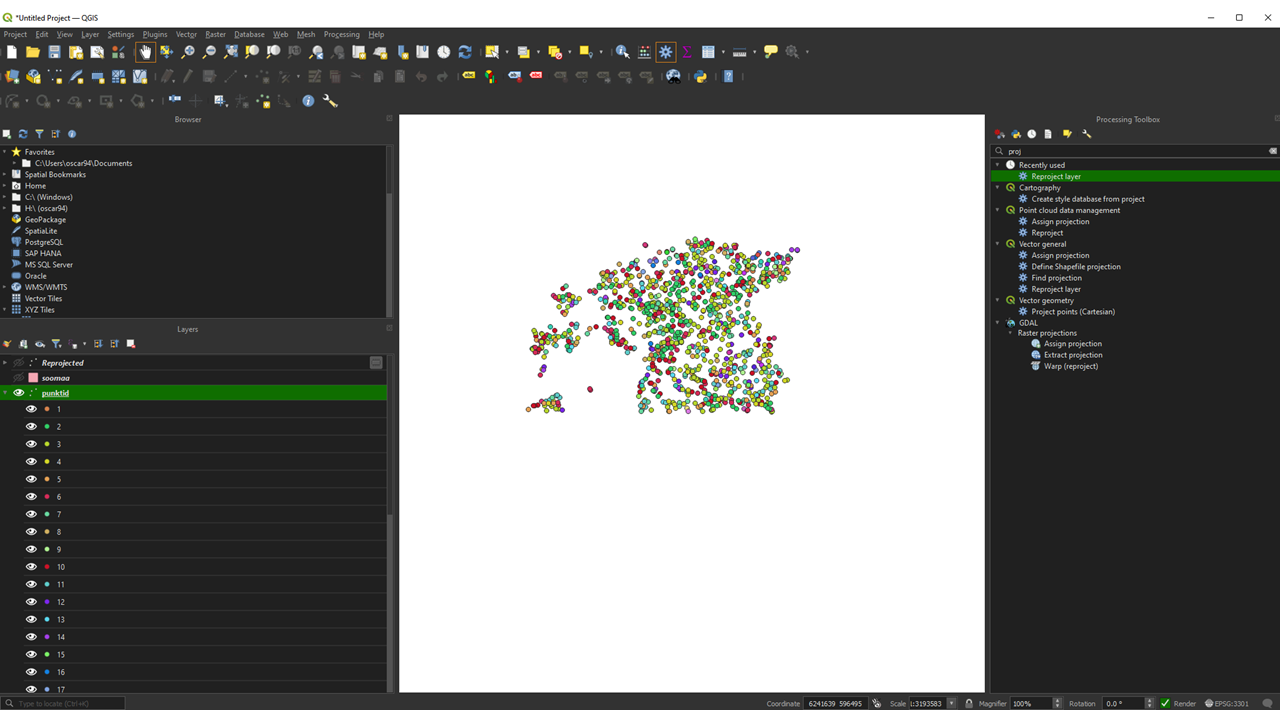
\includegraphics{Lab1/qgis_ss/QGIS_ss12.png}

Try changing the symbology of the soomaa layer and the raster layer

For the raster layer you can try:
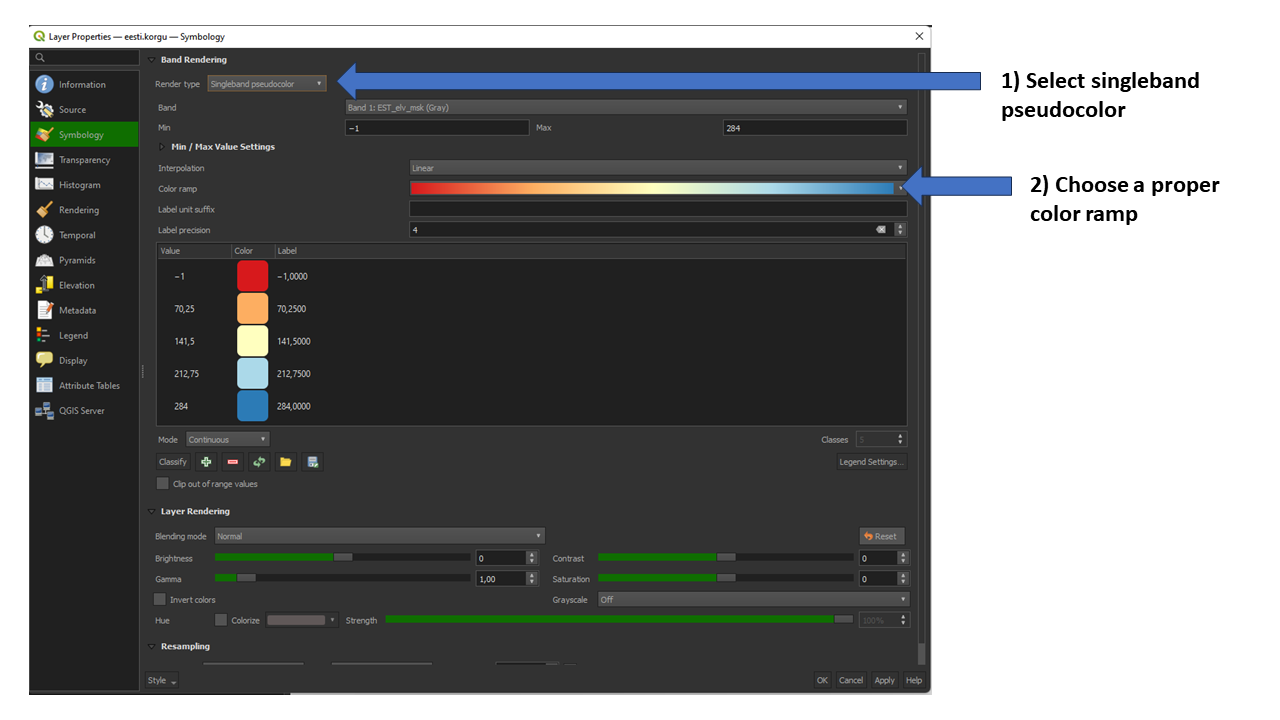
\includegraphics{Lab1/qgis_ss/QGIS_ss13.png}

\hypertarget{iii-set-the-correct-crs-or-projecting}{%
\subsubsection{III) Set the correct CRS or
projecting}\label{iii-set-the-correct-crs-or-projecting}}

\begin{itemize}
\tightlist
\item
  Use the reproject function from the toolbox
\end{itemize}

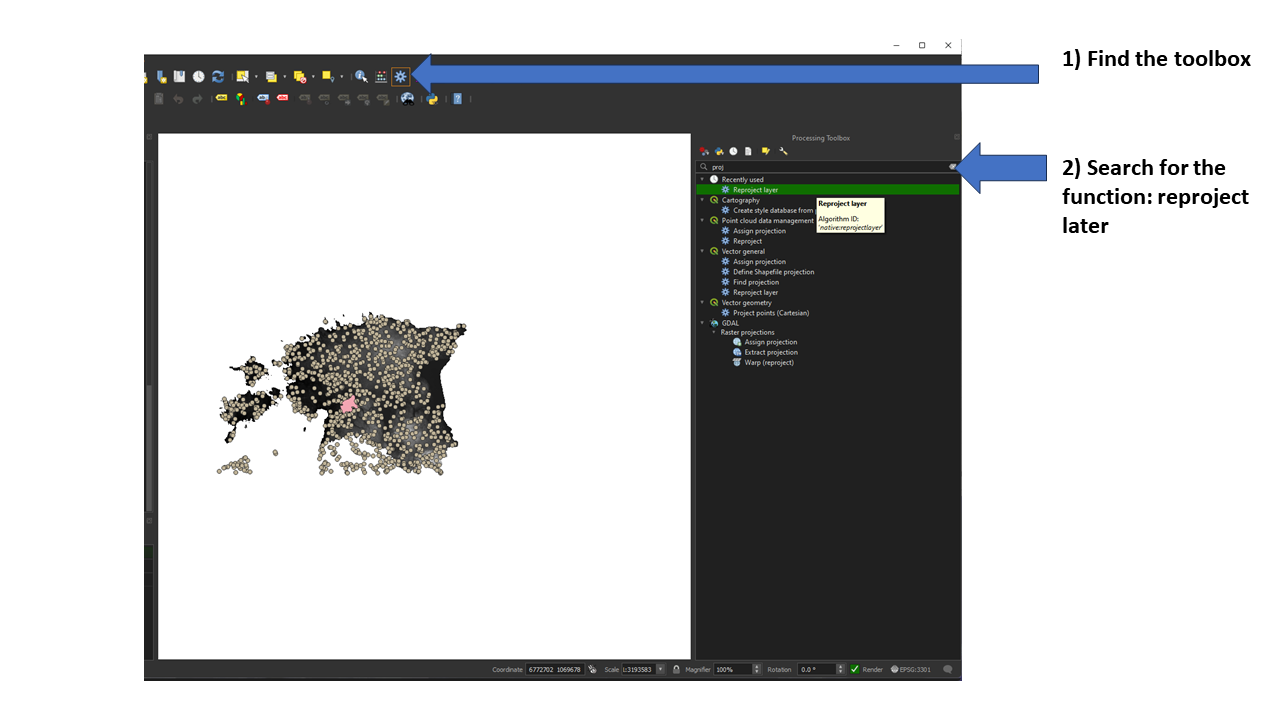
\includegraphics{Lab1/qgis_ss/QGIS_ss8.png}
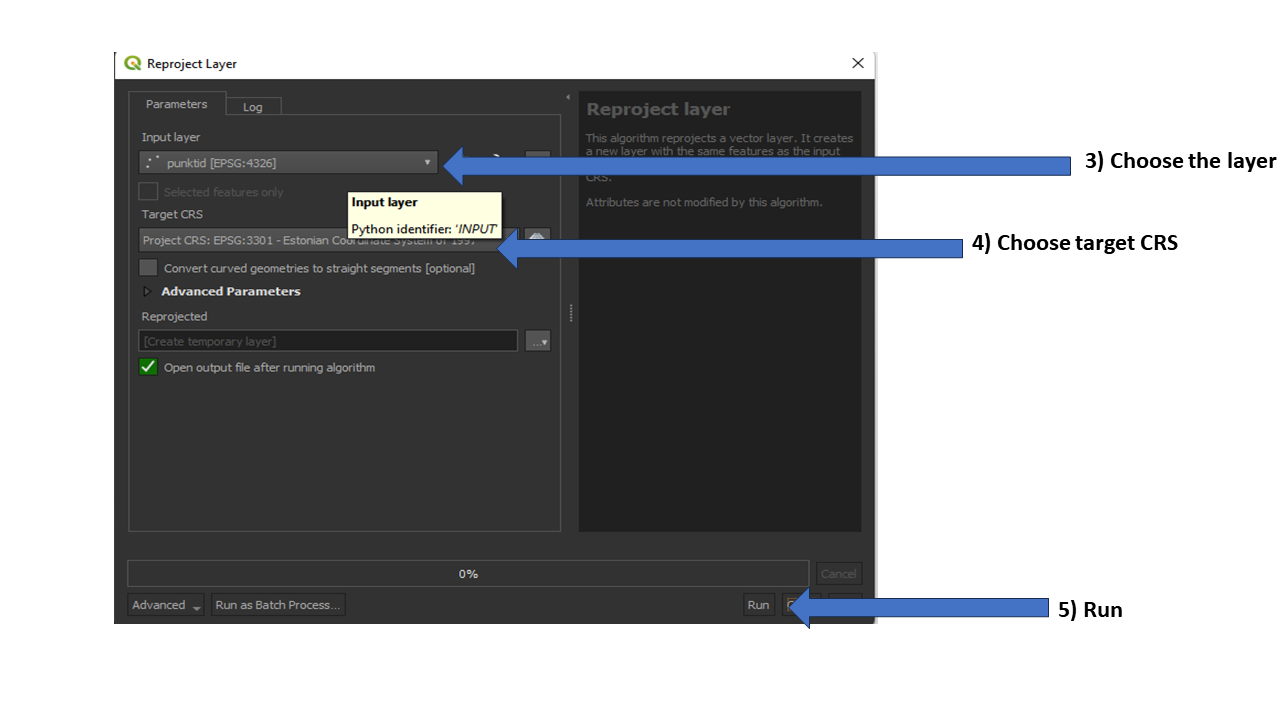
\includegraphics{Lab1/qgis_ss/QGIS_ss9.png}

\begin{tcolorbox}[enhanced jigsaw, colbacktitle=quarto-callout-important-color!10!white, toptitle=1mm, opacityback=0, bottomtitle=1mm, bottomrule=.15mm, leftrule=.75mm, coltitle=black, left=2mm, arc=.35mm, title=\textcolor{quarto-callout-important-color}{\faExclamation}\hspace{0.5em}{Projections}, breakable, colframe=quarto-callout-important-color-frame, opacitybacktitle=0.6, rightrule=.15mm, toprule=.15mm, titlerule=0mm, colback=white]
QGIS projects input layers ``on the fly'' for visualization, the data
does not change. For Spatial Operations you always need to set all
layers on the same CRS. As a good practice always save your reprojected
layers
\end{tcolorbox}

Reproject if necessary your layers. There is a function for reprojecting
vector data, and a different one for raster data.

\hypertarget{iv-spatial-join}{%
\subsection{IV) Spatial Join}\label{iv-spatial-join}}

From the \textbf{ToolBox} find \textbf{Extract by location}

Follow this guide:

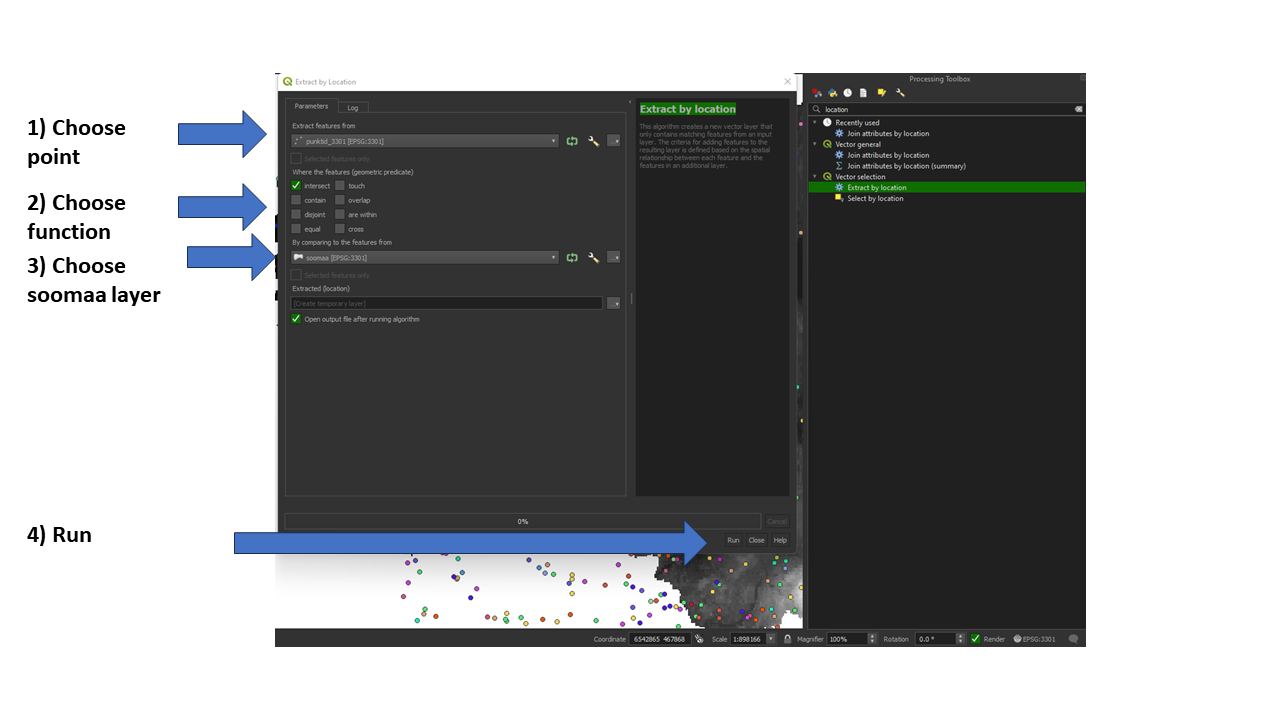
\includegraphics{Lab1/qgis_ss/QGIS_ss14.png}

You can look that a new layer appears. Open the attributes table and
look how many points are there.

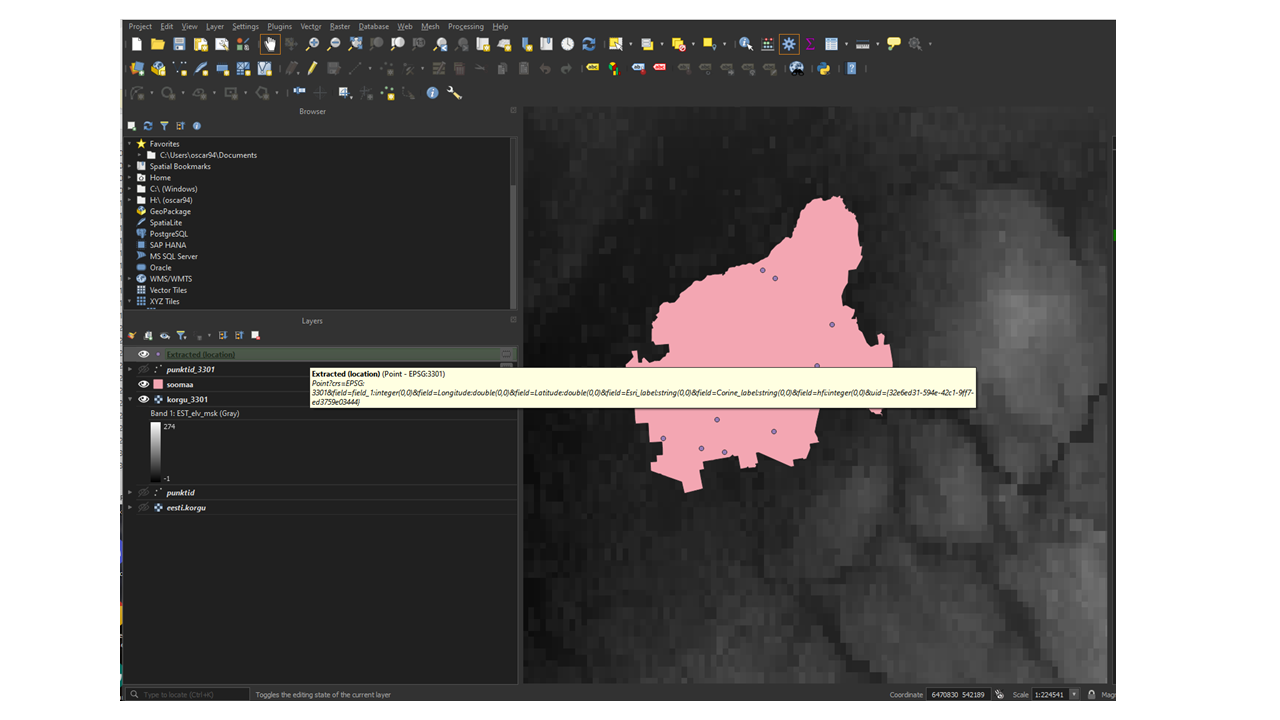
\includegraphics{Lab1/qgis_ss/QGIS_ss15.png}

\begin{tcolorbox}[enhanced jigsaw, colbacktitle=quarto-callout-tip-color!10!white, toptitle=1mm, opacityback=0, bottomtitle=1mm, bottomrule=.15mm, leftrule=.75mm, coltitle=black, left=2mm, arc=.35mm, title=\textcolor{quarto-callout-tip-color}{\faLightbulb}\hspace{0.5em}{}, breakable, colframe=quarto-callout-tip-color-frame, opacitybacktitle=0.6, rightrule=.15mm, toprule=.15mm, titlerule=0mm, colback=white]
Why \textbf{Intersects}?. Check more about
\href{https://postgis.net/docs/using_postgis_query.html\#general-spatial-rel}{\texttt{Spatial\ Queries}}
\end{tcolorbox}

\hypertarget{v-select-by-attribute}{%
\subsection{V) Select by attribute}\label{v-select-by-attribute}}

\begin{itemize}
\tightlist
\item
  Open the attribute table of the target layer (point layer)
\item
  Click on \textbf{Select features using a expression}
  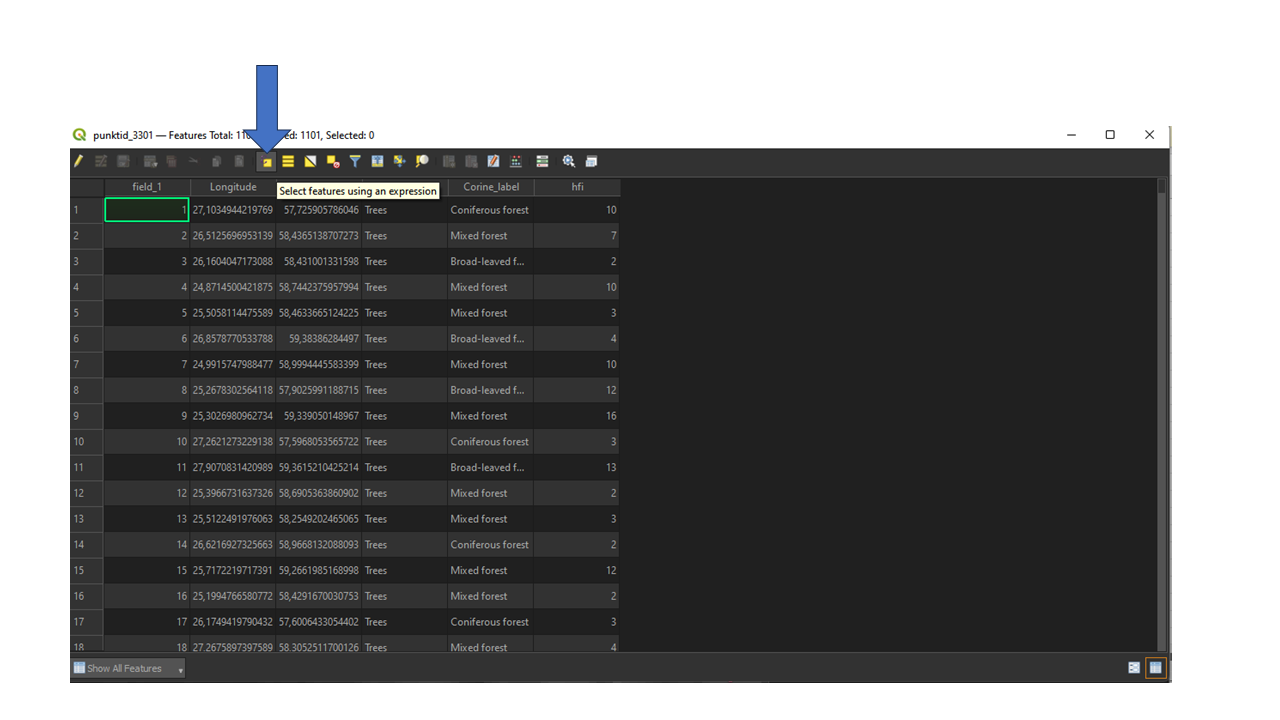
\includegraphics{Lab1/qgis_ss/QGIS_ss16.png}
\end{itemize}

A new window opens. We have to create an expression to select features
(points) based on the Esri\_label column. You can directly write the
expression to filter (QGIS is based on Python), or use the graphical
interface to help you.

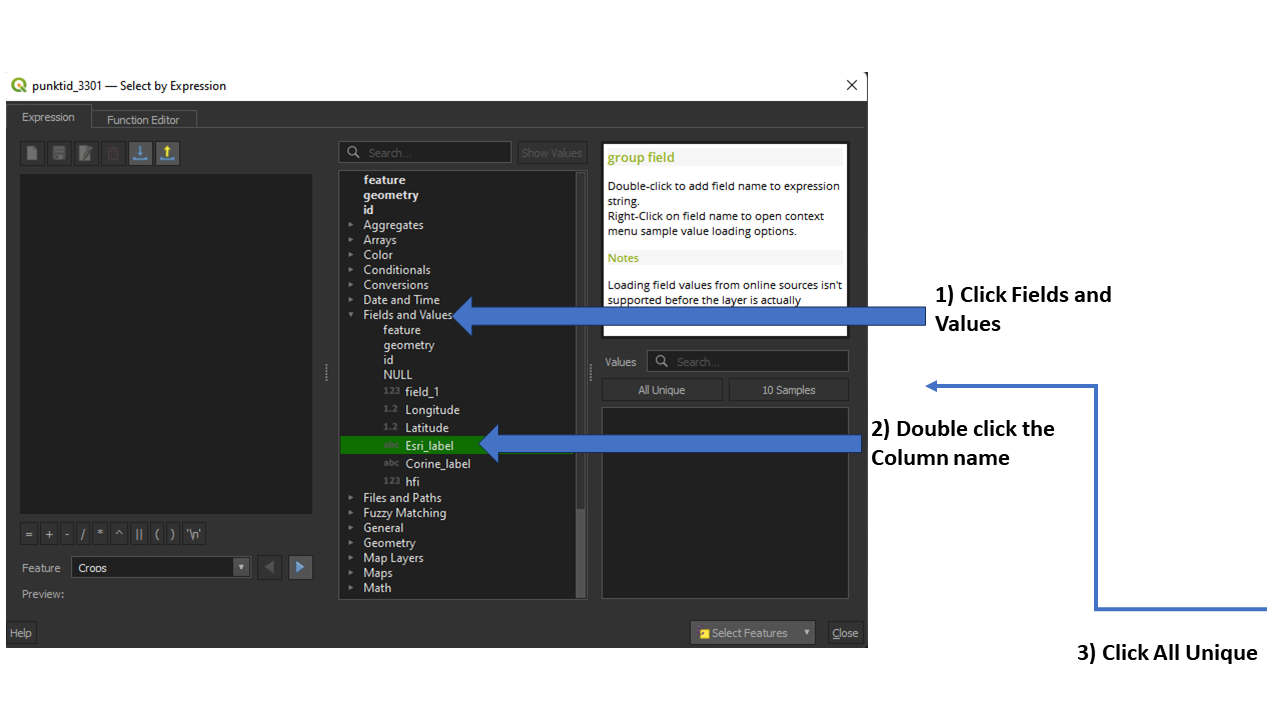
\includegraphics{Lab1/qgis_ss/QGIS_ss17.png}

Write the expression: \textbf{``Esri\_label'' = `Crops'}

And click \textbf{Select Features}

Selected features are highlighted in the attribute table and in the map

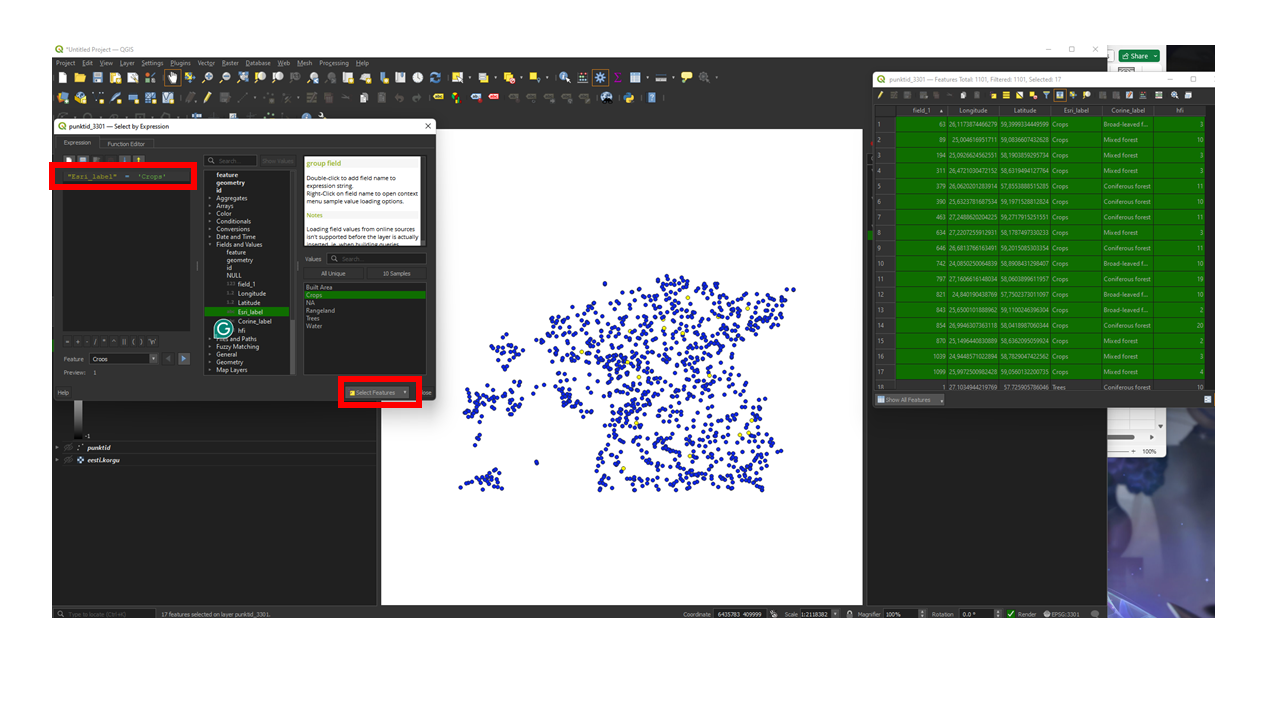
\includegraphics{Lab1/qgis_ss/QGIS_ss18.png}

\begin{itemize}
\tightlist
\item
  Save the selected Features. Right click on the queried layer (points)
  and choose \textbf{Export} - \textbf{Save selected features as}
\end{itemize}

Choose a proper name and directory to save the new layer.

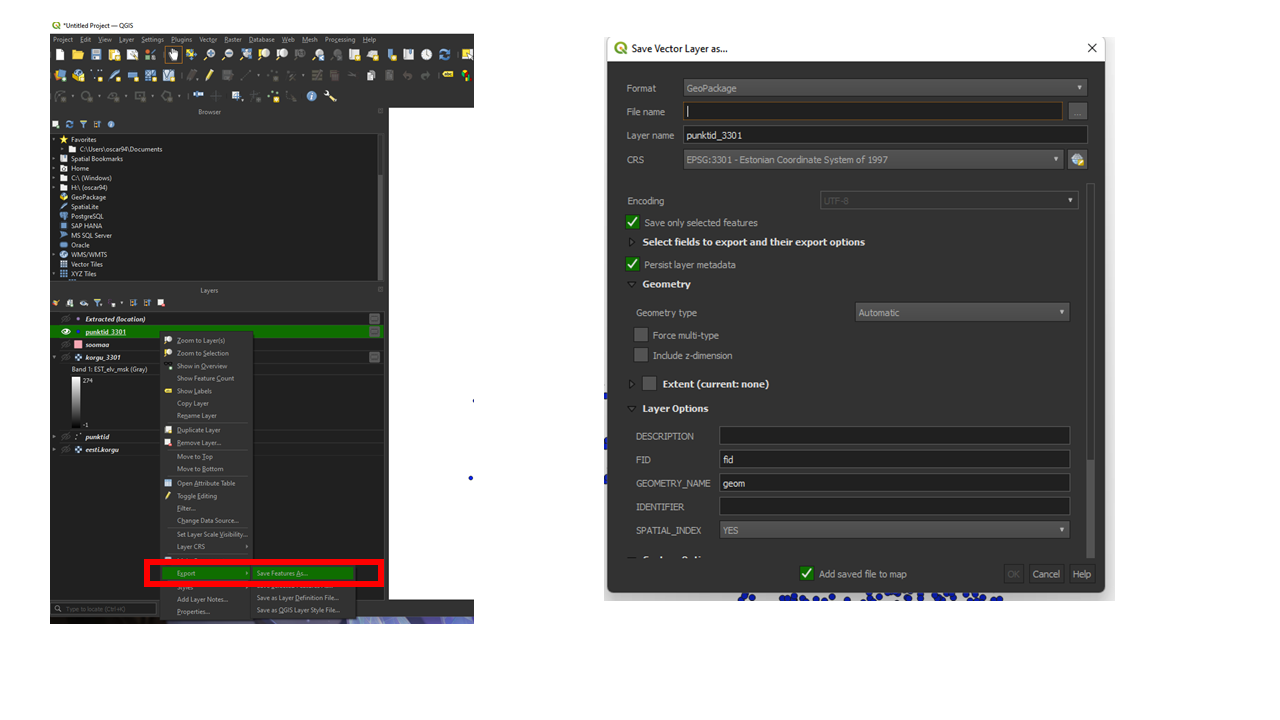
\includegraphics{Lab1/qgis_ss/QGIS_ss19.png}

\hypertarget{vi-buffers}{%
\subsection{VI) Buffers}\label{vi-buffers}}

\begin{itemize}
\item
  Open the points attribute table and select 10 rows.
  \includegraphics{Lab1/qgis_ss/gif_4.gif}
\item
  From the \textbf{ToolBox} find the \textbf{Buffer} function
\item
  Choose the input layer
\item
  Click on the Selected features box
\item
  Fill with the desired distance and set the units
\item
  Run
\end{itemize}

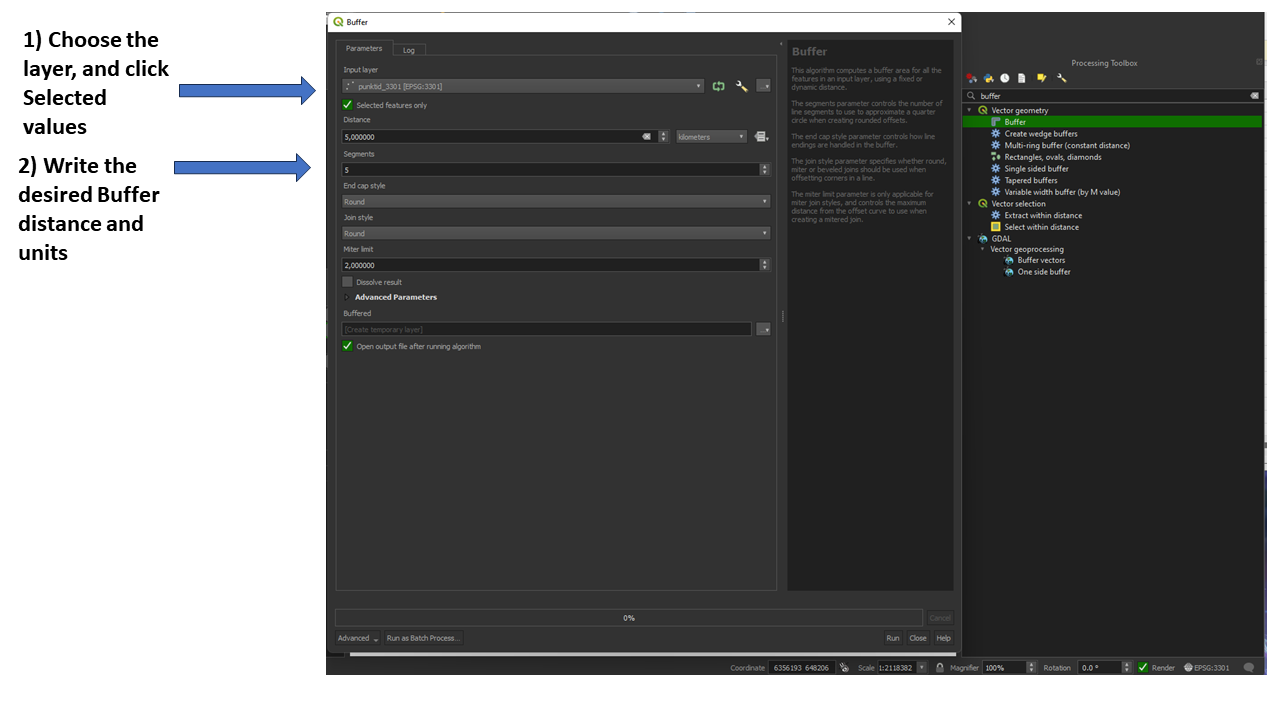
\includegraphics{Lab1/qgis_ss/QGIS_ss20.png}

A new layer will be created (virtual, if you need it later you have to
save it)

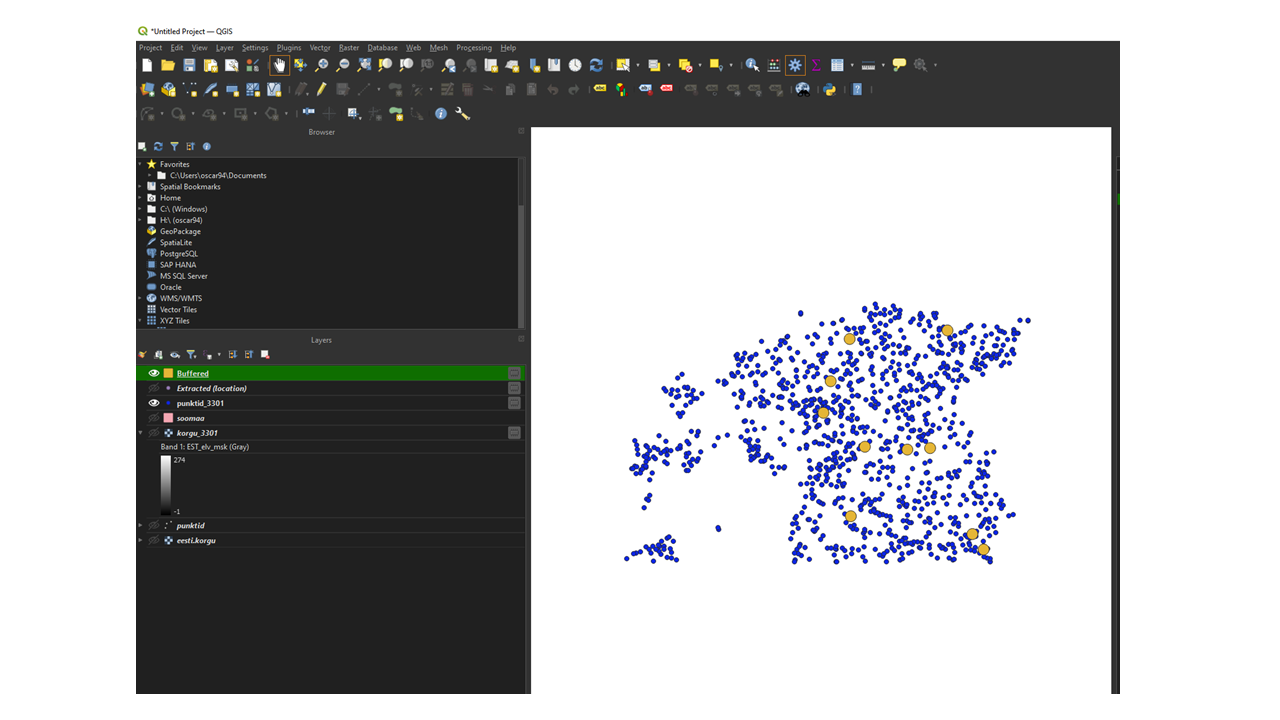
\includegraphics{Lab1/qgis_ss/QGIS_ss21.png}

\hypertarget{vii-field-calculator}{%
\subsection{VII) Field calculator}\label{vii-field-calculator}}

To calculate the buffers areas we need the \textbf{Field calculator}

\begin{itemize}
\tightlist
\item
  Open the attribute table of the Buffers layer
\item
  Click on \textbf{Field calculator} or Ctrl+i
\end{itemize}

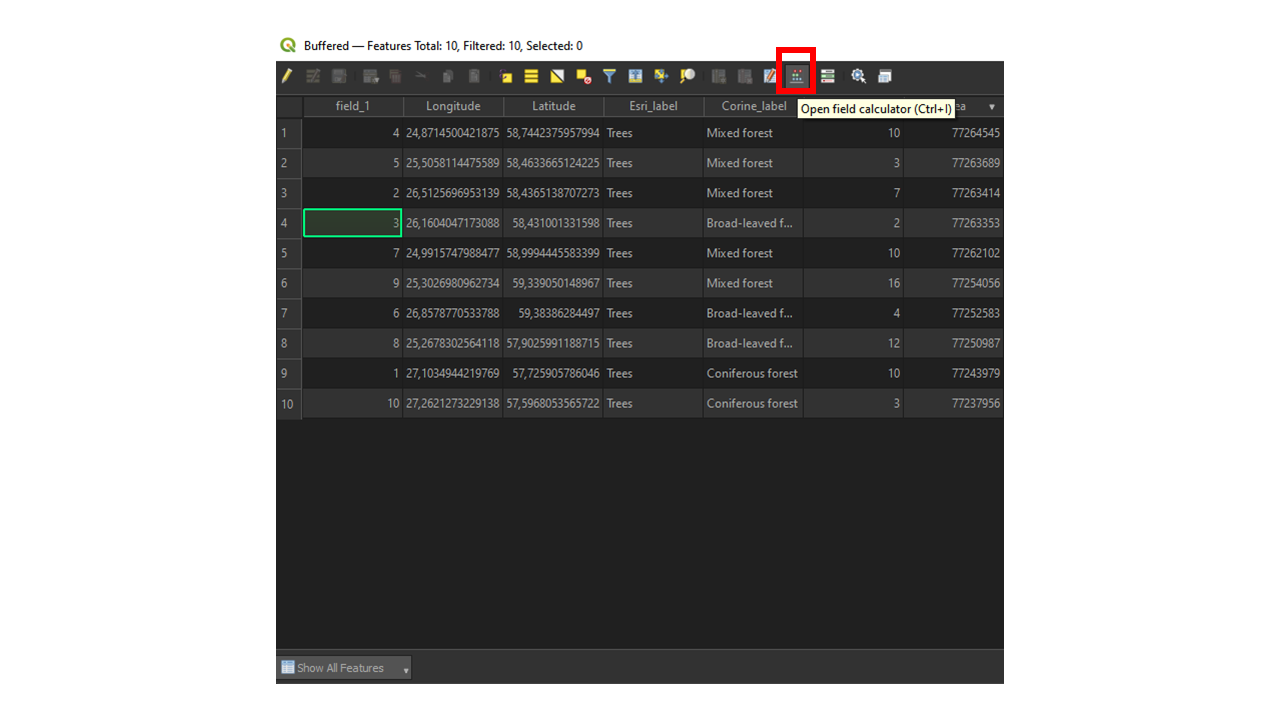
\includegraphics{Lab1/qgis_ss/QGIS_ss22.png}

\begin{itemize}
\tightlist
\item
  Create a new field to store the area
\item
  Look for the function \textbf{\$area}
\item
  OK
\end{itemize}

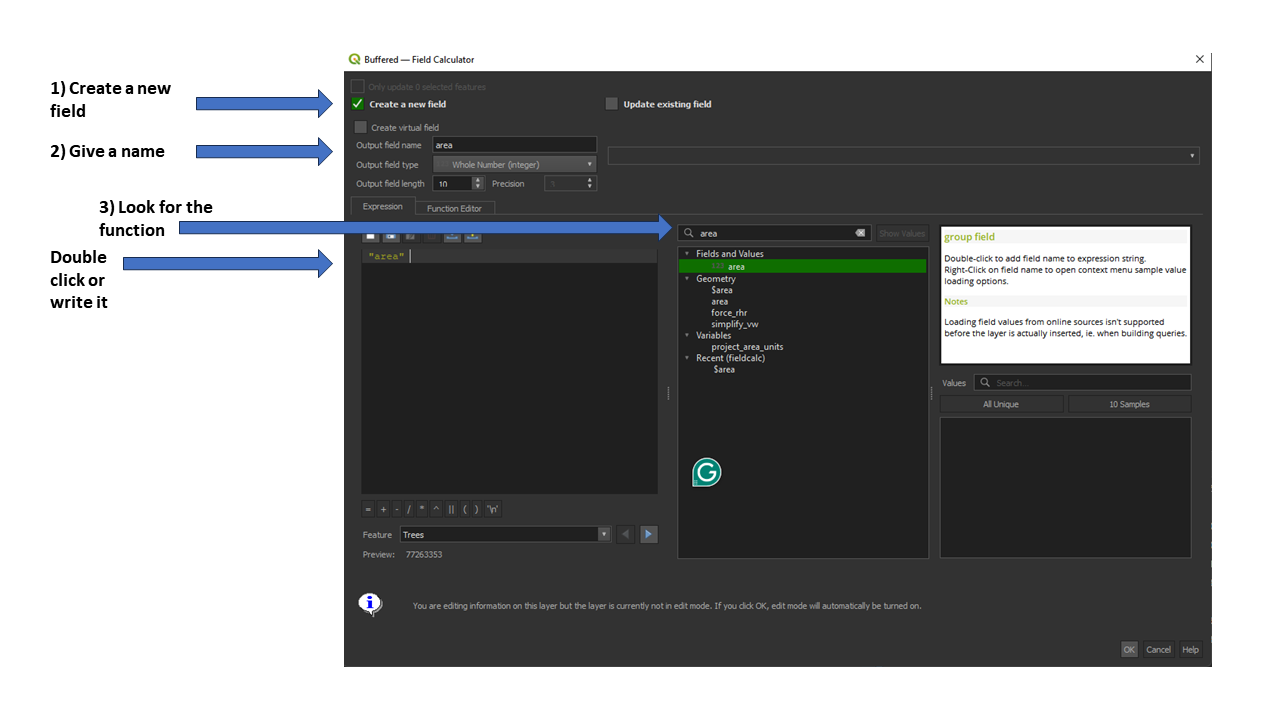
\includegraphics{Lab1/qgis_ss/QGIS_ss23.png}

\begin{itemize}
\tightlist
\item
  A new column is created in the attributes table
\end{itemize}

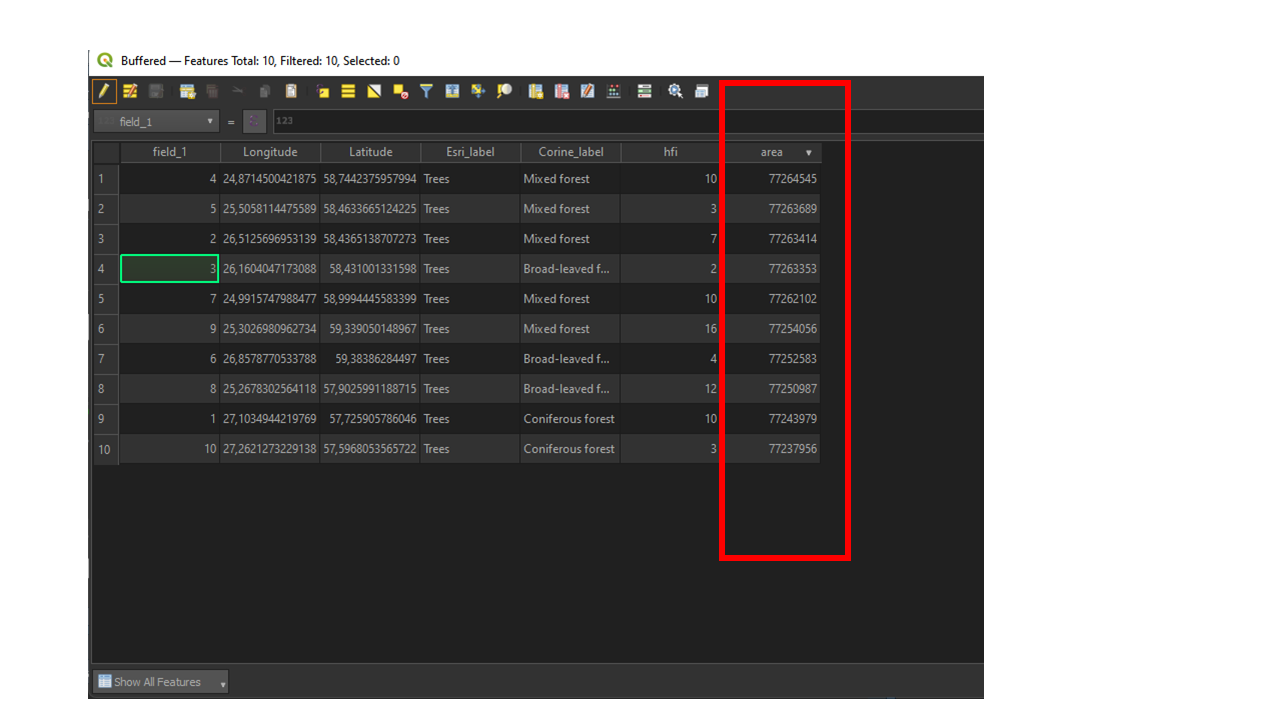
\includegraphics{Lab1/qgis_ss/QGIS_ss24.png}

\hypertarget{viii-raster-data}{%
\subsection{VIII) Raster data}\label{viii-raster-data}}

\hypertarget{clip-raster-using-soomaa-vector}{%
\paragraph{Clip raster using Soomaa
vector}\label{clip-raster-using-soomaa-vector}}

\begin{itemize}
\tightlist
\item
  Find from the \textbf{ToolBox} the function \textbf{Clip Raster by
  Mask Layer}
\item
  Select the input (the raster layer)
\item
  Select the mask (soomaa layer)
\item
  Run
\end{itemize}

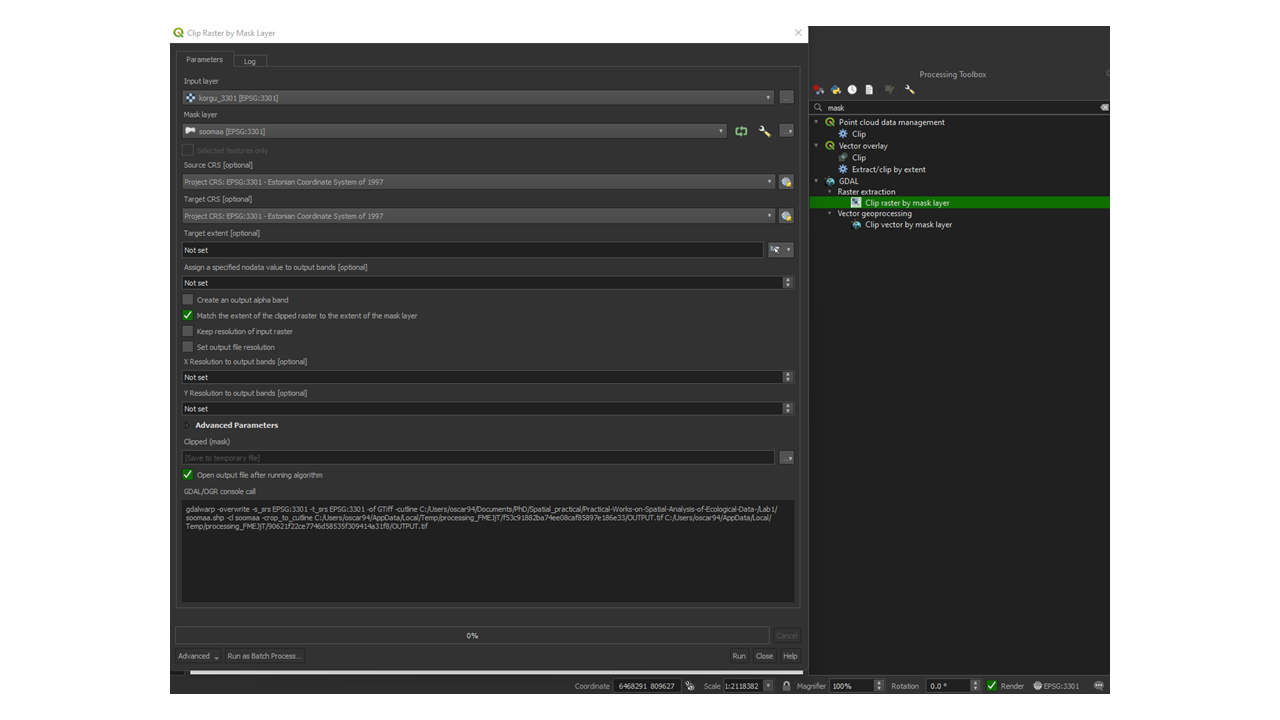
\includegraphics{Lab1/qgis_ss/QGIS_ss25.png}

\begin{itemize}
\tightlist
\item
  The new Clipped layer is created. Remenber to save it if needed in the
  future
\end{itemize}

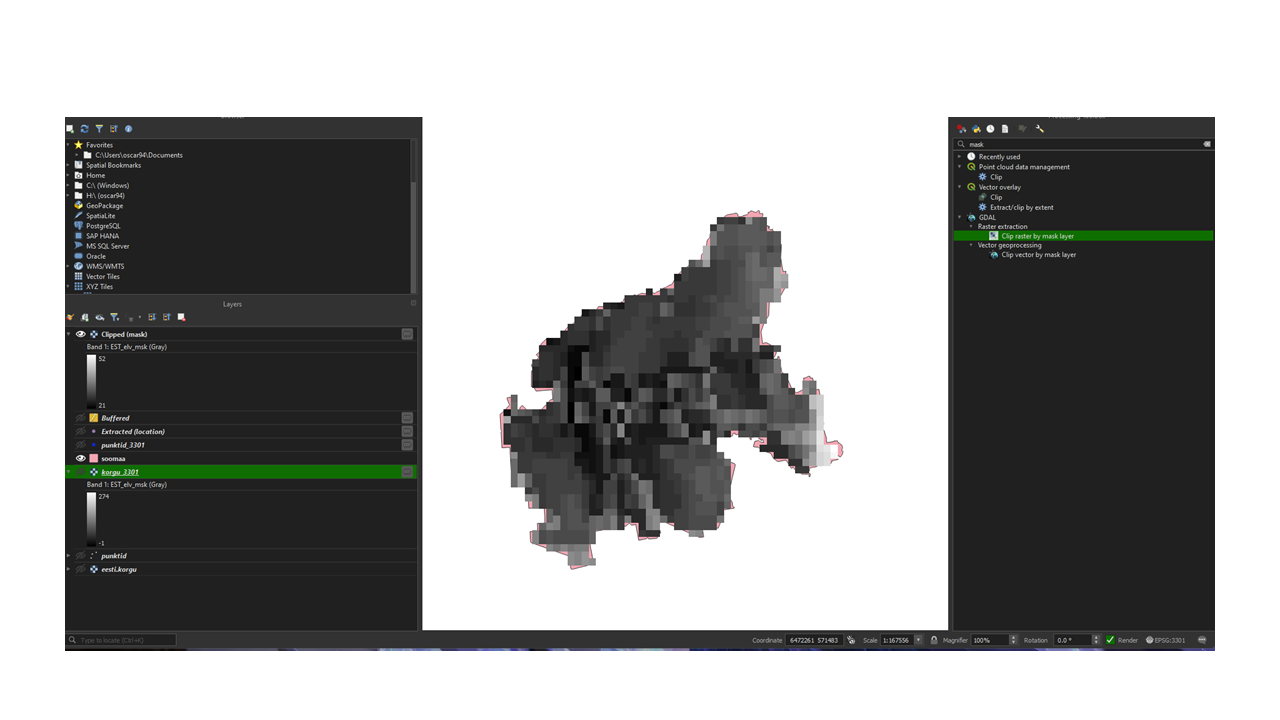
\includegraphics{Lab1/qgis_ss/QGIS_ss26.png}

\hypertarget{raster-layer-statistics}{%
\paragraph{Raster layer statistics}\label{raster-layer-statistics}}

Get basic information of your clipped raster layer

\begin{itemize}
\tightlist
\item
  From the \textbf{ToolBox} look for \textbf{Raster layer statistics}
\item
  Open the summary
\end{itemize}



\end{document}
